
\section{Lepton Identification}
The following three sections briefly describe how certain subsystems of the CMS detector work together to identify muons, electrons, and tau leptons. 

\subsection{Muon Identification Systems}

In order to identify good muons, several subdetector work together to reconstruct muons. Looking at muons that come from the interaction vertex --- prompt muons --- the tracker plays an important role in identifying charged particle tracks. 

As CMS implies in its name, muons are certainly a focal point in particle detection. 

The tracker system works in tandem with the gas chambers to reconstruct muons, and the solenoid measures charge particle's momentum allowing for an accurate mass resolution.  


During reconstruction, tracker or global muons are identified and are ultimately divided into four sub types depending on the $\chi^2$ of the track and momentum of the candidate muon ~\cite{CMS-PAS-PFT-09-001,Kratschmer:1956760}


\subsection{Electron Identification Systems}

The main sub detector system that is involved with electron identification is the ECAL. To identify electrons a cluster of energy in the ECAL is associated with a track that is constructed in the silicon detector system. 

The tracks are identified in the typical fashion by using the Kalman Filter tracking technique to pick good quality tracks, then the tracks are refitted using a Gaussian Sum Filter (GSF). 
This track would then be associated with the ECAL super cluster (SC) by requiring matching in $\eta,\;\phi$ space
\[|\Delta\eta| = |\eta_{\text{SC}} - \eta_{\text{in}}^{\text{extrap}}| < 0.02\]
\[|\Delta\phi| = |\phi_{\text{SC}} - \phi_{\text{in}}^{\text{extrap}}| < 0.15\]
This association amounts to an overall efficiency of about 93\% ~\cite{Khachatryan:2015hwa}. 


%In 2016 better calibration studies were completed at lower energy increasing the ECAL performance and the pixel upgrade in 2017 helped track reconstruction resulting in better electron identification ~\cite{Micheli:2727506}.


\subsection{Tau Identification Systems}
Tau leptons are one of the most diverse particles in the Standard Model, decaying in many different ways. It is the heaviest lepton, so heavy that even tau decays to intermediate mesons are possible. The $\rho$, $a$, and $\pi$ mesons are several possible mesons that the tau can decay to. Therefore, when it comes to tau identification many subsystems are needed to properly identify them in addition to higher level algorithms. The focus of this section is on the hardware components that are needed to identify tau leptons. Tau leptons decay both hadronically and leptonically as shown in the table below \ref{tab:taudecay}. 



\begin{table}[h!tbp]
\centering
    \topcaption{Possible hadronic tau decays ~\cite{Workman:2022}}
\label{tab:taudecay}
\begin{tabular}{c  c r}
Decay Modes & Resonance & \multicolumn{1}{c}{$\mathcal{B}(\%)$} \\\hline
Leptonic Decay && \multicolumn{1}{l}{35.2}\\
$\tau^- \rightarrow e^- \bar{nu}_e \nu_\tau $ & & 17.8 \\
$\tau^- \rightarrow \mu^- \bar{nu}_\mu \nu_\tau$ & & 17.4 \\\hline
Hadronic Decay && \multicolumn{1}{l}{64.8}\\
$\tau^- \rightarrow h^-\nu_\tau$ & & 11.5 \\
$\tau^- \rightarrow h^-\pi^0 \nu_\tau$ & $\rho(770)$ & 25.9 \\
$\tau^- \rightarrow h^-\pi^0 \pi^0 \nu_\tau$ & $a_1(1260)$ & 9.5 \\
$\tau^- \rightarrow h^- h^+ h^- \nu_\tau$ & $a_1(1260)$ & 9.8 \\
$\tau^- \rightarrow h^- h^+ h^- \pi^0 \nu_\tau$ & & 4.8 \\
Other & & 3.3 \\\hline
\end{tabular}
\end{table}

%The important algorithms directly related to hardware are the Hadron Plus Strips (HPS) algorithm which combines the use of the tracker system and the electromagnetic calorimeter (ECAL) for hadronic tau identification ~\cite{Sirunyan_2018}.  

The Hadron Plus Strips (HPS) combines the use of the tracker system and the electromagnetic calorimeter (ECAL) for hadronic tau identification ~\cite{Sirunyan_2018}.  


 


\section{Data and Simulation Used for Analysis}
Data gathered at CMS is organized primarily on the trigger implemented to identify events. For this analysis, requiring muons is paramount and the search should be inclusive. Therefore datasets published by CMS that are considered are single muon, double muon, and electron plus photon datasets depending on the year. These datasets contain the triggers that are the most important for event selection. Single muon triggers that contain isolated muons at 24 and 27 GeV thresholds are implemented, along with double muon triggers with good reconstructed muons that have 17 GeV threshold. More information on triggers and selection will be given in the event selection section. 

The simulation used to compare to data typically use MadGraph5@NLO along with a PYTHIA 8 hadronizer. These CMS-centrally generated samples are then digitized to the same format as real data events collected and processed at CMS high level trigger. These raw data formats are then reconstructed to physics objects - like tracks and higher level objects like muons and $\tau$leptons. A direct comparison between data and simulation can then be made after calibrating simulation in control regions. 

Data taken from CMS during the entire Run II period was examined. This corresponds to 137 $\text{fb}^{-1}$ of integrated luminosity. The list for data and simulation Monte Carlo(MC) is exhaustive and listed in the appendix \ref{app:data}.   

For the MC production of the signal samples, to reflect the 2HDM modeling, events were generated at tree level for a pseudoscalar Higgs like boson between the masses of 15 and 60 in intervals of 5 GeV with gluon fusion production. These masses are sufficient for the parametric modeling described in the fit to obtain a more precise peak resolution. The signal samples were privately produced for 2017 and 2018, because CMS MC generator contacts weren't sufficient in providing the samples in an acceptable manner. Sampled existed from the 2016 analysis. 
MadGraph5@NLO v2.6.5 was used to generate these events with a PYTHIA 8 hadronizer. Privately produced samples were used for 2017 and 2018. However, the scripts and conditions used are located here:
 \texttt{https://github.com/samhiggie/iDM-analysis-AODproducer/tree/haa} .
The NMSSMHET model was used to simulate the events. Parameters and information can be seen in the package:
https://cms-project-generators.web.cern.ch/cms-project-generators/ .



\subsection{2 $\mu$ 2 $\tau$ Signal Samples }
For the Monte Carlo production of the signal samples, to reflect the 2HDM modeling, events were generated at tree level for a pseudoscalar Higgs like boson between the masses of 15 and 60 in intervals of 5 GeV with gluon fusion production. These masses are sufficient for the parametric modeling described in the fit to obtain a more precise peak resolution.
MadGraph5@NLO v2.6.5 was used to generate these events with a PYTHIA 8 hadronizer. Privately produced samples were used for 2017 and 2018. However, the scripts and conditions used are located here:
 \texttt{https://github.com/samhiggie/iDM-analysis-AODproducer/tree/haa} .
The NMSSMHET model was used to simulate the events. Parameters and information can be seen in the package:
https://cms-project-generators.web.cern.ch/cms-project-generators/ .
 


\section{Corrections to Simulations }

%corrections.TeX
For accurate results that reflect true experimental data, many corrections to MC samples are made. In general, in compliance with CMS's Physics Object Groups (POGs), standard techniques are applied to ensure proper simulation. Of critical importance is the corrections to energy scales for the leptons in the analysis. These corrections will affect the nominal energy recorded for the event as well as the rates in which objects are identified.  In order to protect against bias and to investigate systematic errors, corrections that could effect the results are considered in the overall error in the statistical inference model.

\subsection{Muon energy scale}
Corrections to the muon's energy scale are computed for the muons that pass selection for the analysis. Medium muon ID with track based isolation that pass the isolated single muon triggers at 24 GeV and 27GeV are then rescaled for pileup, efficiency, di-lepton $P_T$ and EWK re-weighting of based on accurate gauge boson measurements. After selection, the scale factors for energy corrections are measured and parametrized in $\phi$ and $\eta$ in multiplicative and additive corrections 
\[\rho^{\text{cor}}=\kappa(\eta,\phi)\rho+Q \lambda(\eta,\phi)\] 

In practice these are just scale factors applied to the energy scale in certain eta phi regions. \\
\begin{table}[h]
  \begin{center}
    \topcaption{Measured \Pmu energy scale correction for genuine \Pmu across all years.}
    \label{tab:MES}
    \begin{tabular} { l | c }
      \hline \multicolumn{2}{c}{Correction (\%)} \\
      \hline $\eta$ region & scale factor  \\ \hline
      $0 - 1.2$ & $0.4$ \\ 
      $1.2 - 2.1 $& $0.9 $\\ 
      $> 2.1$ & $2.7$ \\ 
    \end{tabular}
  \end{center}
\end{table}\\

\subsection{Electron energy scale}

Genuine electron energy scale and resolution requires corrections to be applied to MC in order to match data ~\cite{EGammaEnergyScale}. These corrections are provided directly by the E/Gamma POG, and applied to genuine electrons coming from tau lepton decays for the channels $\mu\mu e \mu$ and $\mu\mu e \tau$.

The energy shift is split depending on the $\eta$ of the electron shown in table \ref{tab:EES}.\\
\begin{table}[h]
  \begin{center}
    \topcaption{Measured \Pe energy scale correction for genuine \Pe across all years.}
    \label{tab:EES}
    \begin{tabular} { l | c }
      \hline \multicolumn{2}{c}{Correction (\%)} \\
      \hline $\eta$ region & scale factor  \\ \hline
      $0 - 1.2$ & $1.0$ \\ 
      $1.2 - 2.1 $& $1.0 $\\ 
      $> 2.1$ & $2.0$ \\ 
    \end{tabular}
  \end{center}
\end{table}\\

\subsection{$\tau$ energy scale}
There is a central energy shift based on the type of tau decay. Due to the electroweak interactions $\tau$ leptons decay hadronically and leptonically. Figure \ref{fig:taudecay} shows the typical tau decay leptonically or hadronically.  \\

\begin{figure}[ht!b]
\begin{center}
  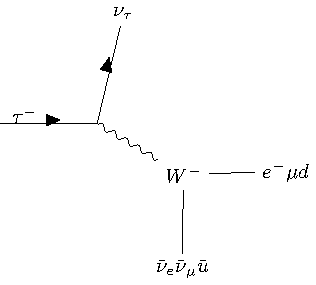
\includegraphics[width=0.47\textwidth]{"Figures/taudecay.pdf"}
    \caption{\label{fig:taudecay} diagram depicting the possible decays of the tau lepton: 65\% of the time hadronically and 18\% to tau neutrino and electron with antielectron neutrino (17\% for muon)}
\end{center}
\end{figure} 
When the tau decays hadronically, many different intermediate mesons are produced and each type of decay has different kinds of signatures particularly when they hadronize and deposit the energy within the hadronic calorimeter of CMS. The Tau-POG has measured the central value systematic deviation as a form of scalar factor that should be applied for an accurate result of measuring the tau's energy. This is split by the prongs (charged hadrons) and $\pi^0$ s.  

\begin{table}[h]
  \begin{center}
    \topcaption{Measured $\tauh$ energy scale correction for genuine $\tauh$'s across all years.}
    \label{tab:TES}
    \begin{tabular} { l | c  c  c }
      \hline \multicolumn{4}{c}{Correction (\%)} \\
      \hline Decay mode & 2016 & 2017 & 2018 \\ \hline
      $h^{\pm}$ & $-0.6$ & $0.7$ & $-1.3$  \\ 
      $h^{\pm}\pi^{0}$ & $-0.5$ & $-0.2$ & $-0.5$  \\ 
      $h^{\pm}h^{\pm}h^{\pm}$ & $0.0$ & $0.1$ & $-1.2$ \\ 
    \end{tabular}
  \end{center}
\end{table}

The deviation in the model is measured by between the difference in data and MC for different values of hadronic tau energy. The uncertainty is measured for each decay mode considered in the analysis. Figures \ref{fig:taues} shows the differences in data and MC for the 1 prong + $\pi_0$ decay mode as a function of tau energy, all other tau decay modes are also measured. 

\begin{figure}[h!]
    \begin{center}
        \includegraphics[width=0.32\textwidth]{Figures/TauPOG/mtau_1ProngPi0_nominal_v3.pdf}
        \includegraphics[width=0.32\textwidth]{Figures/TauPOG/mtau_1ProngPi0_minus6percent_v3.pdf}
        \includegraphics[width=0.32\textwidth]{Figures/TauPOG/mtau_1ProngPi0_plus6percent_v3.pdf}
    \end{center}
    \caption{Tau mass distributions considering the nominal $\tau_h$ energy scale in simulation (left), or the $\tau_h$ energy scale shifted by -6 (left) or +6\% (right), in the $\mu\tau_h$ final state, for the 1 prong + pizero decay mode.}
    \label{fig:taues}
\end{figure}

\subsection{$\tauh$ ID efficiency}

Genuine $\tauh$ identification efficiency can be different in Data and MC ~\cite{TAUIDTwiki}. To correct for this difference, measurements are 
made in an inclusive $\mu\tau$ channel, using genuine Drell-Yan to $\tauh$ as a signal and using the invariant mass
of the $\Pgm\tauh$ as an observable. Naturally, this region has far more statistics than the control and signal regions in the pseudoscalar analysis. To measure the identification efficiency precisely, it is done in the inclusive regions with an emphasis of simulation containing real taus. This measurement is done by the Tau POG, and the scale factors are provided to CMS. 

For the $\mu\mu e \tauh$ and $\mu\mu\mu\tauh$ channels, scale factors are binned in 3 different $\pt$ bins: 30--35, 35--40, and 40+ \GeV. In the $\tauh\tauh$ final state, the efficiencies are also binned by decay mode. 


These efficiencies, while used in the primary event and the parameter of interest in the fit, they are not considered in the systematic model as they are expected to have very little impact on fit and limits based on the 2016 result. 


\subsection{$e \rightarrow \tauh$  and $\mu \rightarrow \tauh$ misidentification rate}
The efficiencies associated with $\tau$ identification through the Deep Neural Net approach is considered. 
The efficiency of the discriminators against electrons or muons misidentified as $\tauh$ candidates can be miss-modeled in simulation. 
These data/MC scale factors are
binned by barrel/endcap region of the measured $\eta_{\tauh}$, and by $\tauh$ decay mode. They depend on the anti-electron or anti-muon discriminator used. 
Scale factors are measured to correct this and are applied to $\Pe \rightarrow \tauh$ in MC. Full information on misidentification measurements and application in analyses can be found in reference ~\cite{TAUIDTwiki}. 


The misidentification scale factors are derived by pass and fail regions. The regions are set up by selecting events where a reconstructed $\tauh$ passes the DNN working point and also fails the DNN discriminant against muons. QCD multijet is estimated from same sign lepton region within data - similar to the fake rate calculation like in chapter \ref{chap:background}. W+Jets normalization is carefully selection from a region with high transverse mass. The visible mass distributions of the events in these regions are fit and the overall signal yield remains constant in the pass and fail regions. The normalization of $Z \to e e $ background is allowed to vary in this muon faking tau measurement.   
The expected impact on the systematic model from these anti-lepton discriminators are expected to be very small so they are not included in the uncertainty model.

%The scale factors are obtained by separating events with a reconstructed muon and a reconstructed $\tauh$ passing
%the deep tau ID into a category where the $\tauh$ passes or fails the discriminator against muons. All the processes in
%these regions are taken from simulation, except the QCD multijet background, which is estimated from SS data, and the W+jets background, which is normalized in a region with high $m_T$. The visible mass distributions in the pass and fail regions are fitted using the $e\to\tauh$ scale factor as parameter of interest. An increase of the POI causes an increase of the signal yield in the pass region and simultaneously a decrease of the signal in the fail region, such that the signal yield in the two regions combined is unchanged. 
%Additionally, the normalization of the $\PZ\to\Pe\Pe$ background is freely floating to modelna scale
%factor related to applying the discriminator against jets to muons. The scale factor applied to muons faking taus in the 
%analysis is the product of the scale factor of the discriminator against jets and scale factor of the discriminator against muons.


\subsection{Pileup Re-weighting}

MC events are re-weighted using a minimum bias cross section equal to the luminosity for the corresponding year. This pileup re-weighting is to rescale the events for effective number of primary interactions during collisions. During Run II, pileup or the number of primary vertices in a crossing or underlying event could reach close to 100 and in Run III this will exceed 200.   

\subsection{Electron and muon identification efficiency}

Scale factors derived within the HTT group are applied for muons~\cite{AN16355}, and the EGamma POG scale factors are applied for electrons~\cite{EGammaMVAID}. The scale factors for muons with $5<\pt<9$ GeV and $9<\pt<10$ GeV, are computed privately as there are no official numbers, and were approved by the MuonPOG in the 2016 analysis. 
  
%\subsection{B tagging efficiency}

%The analysis vetoes events with at least one b tagged jet. The scale factors provided by the BTV POG~\cite{btvtwiki} are applied.

\subsection{Generator event weights and luminosity}

Generator weights are applied on an event-by-event basis. Samples produced with the aMCatNLO generator contain both positive and negative event weights. The presence of negative event weights reduces the
effective statistics of the samples.
The event weights for simulation are scaled to the expected yields for each sample. The number
of generated events in each sample is used, however in the aMCatNLO sample this sum of
generated events is weighted by the generator weights, effectively making the aMCatNLO
samples smaller when weighting for luminosity and cross section.
Additionally, K-factors are considered for W+Jets and Drell-Yan samples in order to correct between purely generated events and reconstructed event yeilds for Drell-Yan a factor of 1.1637 is used and for W+Jets a factor of 1.221 is used. These are applied to each exclusive and inclusive samples during the combination of inclusive and exclusive sample processing.   
%\subsection{Trigger weights}
%
%We use a trigger scale factor of 1.0 for the soup of single muon, double muon, and triple muon triggers. This is consistent with what was measured by various analyses, for example in Refs \cite{AN16392}, \cite{AN17020}.
%

\subsection{Offline Muon Selection}
Due to the selection of muons at 5 GeV, which is below the trigger threshold, scale factors were measured in the barrel and encaps using the tag and probe technique in the 2016 analysis. These factors are considered, in addition to the Muon POG's recommendation, to support correct simulation of data. 
\begin{table}[h!tbp]
\centering
\topcaption{Scale factors to correct for Offline muon selection being less than the online trigger threshold. 
\label{tab:event_yield}
}
\begin{tabular*}{0.6\textwidth}{c|c|c}
   & Barrel & Endcap \\\hline
Muons with $5 < pT < 9$ GeV & 0.956 & 0.930\\\hline
Muons with $9 < pT < 10$ GeV & 0.916 & 0.897\\\hline 
\end{tabular*}
\end{table}


\subsection{Visualizing the Corrections}
The energy scales for the various leptons used in the analysis are not only changed in the nominal case, but their uncertainty is measured and then propagated to the fit model via changes in the normalization for the distribution. To visualize this and provide a cross check distributions for the $\tau$ $\mu$ and e energy scales are cross checked in the parameter of interest ( the mass of the di-muon system from the leading pt-pseudoscalar "a" particle). 
These systematics for $\mu\mu\tau\tau$ channel are visualized here in figure \ref{fig:sys_shift_mmtt2016}.
\begin{figure}[ht!b]
  \centering
\includegraphics[width=0.31\textwidth]{Figures/outplots_v7plots_allsys_scale_m_etalt1p2Down/mll_fine_mmtt_inclusive.png} 
\includegraphics[width=0.31\textwidth]{Figures/outplots_v7plots_allsys_Nominal/mll_fine_mmtt_inclusive.png}
\includegraphics[width=0.31\textwidth]{Figures/outplots_v7plots_allsys_scale_m_etalt1p2Up/mll_fine_mmtt_inclusive.png} \\

    \caption{\label{fig:sys_shift_mmtt2016} Systematic Shift in the Uncertainty Model for 2016 $\mu\mu\tau\tau$ for the muon energy scale shift down (left), nominal (mid), and up (right), no data is shown on this plot as it directly reflects the signal region without the extraction cuts }
\end{figure}

In the end, the uncertainty considered in the fit model would then be the percent yield up and down as a log-normal that affects the normalization of the template. Because the model is so statistically limited the log-normal is sufficient in capturing the changes in the distributions over the fit range.  
